\documentclass{standalone}
%outline around text
\usepackage[outline]{contour}
\contourlength{1.3pt}

%tikz
\usepackage{tikz}
\usetikzlibrary{knots, cd, calc}

\begin{document}
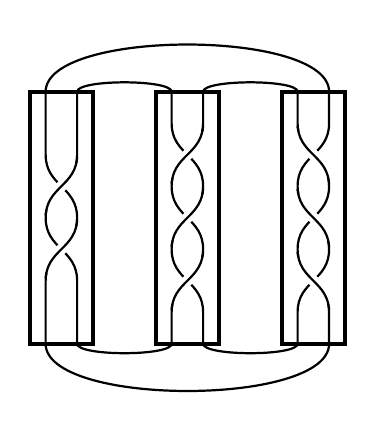
\begin{tikzpicture}[scale = 0.8]

\draw[ultra thick] (0, -0.5) rectangle (1, 3.5);
\draw[ultra thick] (2, -0.5) rectangle (3, 3.5);
\draw[ultra thick] (4, -0.5) rectangle (5, 3.5);

\begin{knot}[clip width = 5, flip crossing/.list={2, 4, 6, 8}]
\strand[thick] (0.25, -0.5) -- (0.25, 0.5) .. controls +(0, 0.5) and +(0, -0.5) .. (0.75, 1.5) .. controls +(0, 0.5) and +(0, -0.5) .. (0.25, 2.5) -- (0.25, 3.5);

\strand[thick] (0.75, -0.5) -- (0.75, 0.5) .. controls +(0, 0.5) and +(0, -0.5) .. (0.25, 1.5) .. controls +(0, 0.5) and +(0, -0.5) .. (0.75, 2.5) -- (0.75, 3.5);


\strand[thick] (2.25, -0.5) -- (2.25, 0) .. controls +(0, 0.5) and +(0, -0.5) .. (2.75, 1) .. controls +(0, 0.5) and +(0, -0.5) .. (2.25, 2) .. controls +(0, 0.5) and +(0, -0.5) .. (2.75, 3) -- (2.75, 3.5);

\strand[thick] (2.75, -0.5) -- (2.75, 0) .. controls +(0, 0.5) and +(0, -0.5) .. (2.25, 1) .. controls +(0, 0.5) and +(0, -0.5) .. (2.75, 2) .. controls +(0, 0.5) and +(0, -0.5) .. (2.25, 3) -- (2.25, 3.5);



\strand[thick] (4.25, -0.5) -- (4.25, 0) .. controls +(0, 0.5) and +(0, -0.5) .. (4.75, 1) .. controls +(0, 0.5) and +(0, -0.5) .. (4.25, 2) .. controls +(0, 0.5) and +(0, -0.5) .. (4.75, 3) -- (4.75, 3.5);

\strand[thick] (4.75, -0.5) -- (4.75, 0) .. controls +(0, 0.5) and +(0, -0.5) .. (4.25, 1) .. controls +(0, 0.5) and +(0, -0.5) .. (4.75, 2) .. controls +(0, 0.5) and +(0, -0.5) .. (4.25, 3) -- (4.25, 3.5);

\strand[thick] (0.75, -0.5) .. controls +(0, -0.2) and +(0, -0.2) .. (2.25, -0.5);
\strand[thick] (2.75, -0.5) .. controls +(0, -0.2) and +(0, -0.2) .. (4.25, -0.5);
\strand[thick] (0.25, -0.5) .. controls +(0, -1) and +(0, -1) .. (4.75, -0.5);


\strand[thick] (0.75, 3.5) .. controls +(0, 0.2) and +(0, 0.2) .. (2.25, 3.5);
\strand[thick] (2.75, 3.5) .. controls +(0, 0.2) and +(0, 0.2) .. (4.25, 3.5);
\strand[thick] (0.25, 3.5) .. controls +(0, 1) and +(0, 1) .. (4.75, 3.5);


\end{knot}
\end{tikzpicture}
\end{document}